\chapter{Chapitre I -- Les Sources (Courant et Tension)}

\section{Signaux}

\subsection{Définitions}
\textbf{Signal} : Grandeur physique qui varie en fonction du temps, de l'espace ou d'autres variables indépendantes. \\
\vspace{5px}
L'existence d'un signal implique qu'un \textbf{phénomène} est à l'origine de sa génération phénomène qui nécessite de l'énergie pour être produit. \\ 
Ce phénomène est mesurable, car le signal transmet une \textbf{information}. \\
\vspace{5px}
\textit{Il existe deux manières d'observer un signal :}
\vspace{5px}
\begin{itemize}
    \item[-] \textbf{Notion Dynamique (I)} : Observation de l'évolution du signal (de l'intensité, du courant électrique) en fonction du temps.
    \item[-] \textbf{Notion Statique (U)} : Observation de la répartition des charges (de la tension / du potentiel) à un instant donné.
\end{itemize}
\vspace{15px}
\subsection{Types de signaux}
On distingue deux types de signaux : \\
\vspace{10px}
\begin{minipage}[htp]{0.45\textwidth}
    \textbf{Signaux variables} : Signaux qui varient en fonction du temps. (eg. ensoleillement) \\
    \begin{center}
        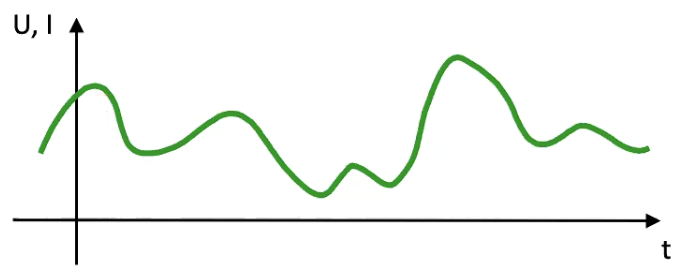
\includegraphics[width=\textwidth]{chapters/chapter1/images/variable.png}
    \end{center}
\end{minipage}
\hfill
\vline
\hfill
\begin{minipage}[htp]{0.45\textwidth}
\textbf{Signaux continus} : Signaux constants au cours du temps. (eg. une pile) \\
\begin{center}
    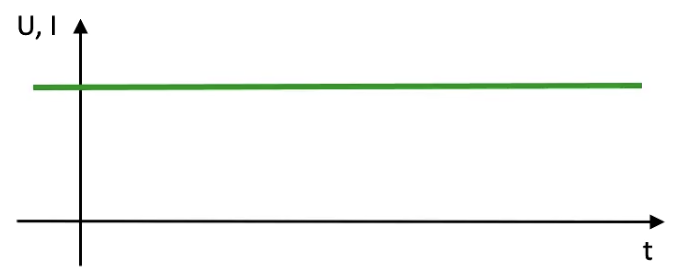
\includegraphics[width=\textwidth]{chapters/chapter1/images/continu.png}
\end{center}
\end{minipage}
\newpage
\subsection{Signaux alternatifs et périodiques}
\textbf{Signal alternatif} : Signal qui change de signe à intervalles réguliers. \\ 
\textbf{Signal périodique} : Signal qui se répète à intervalles réguliers. \\

\begin{center}
    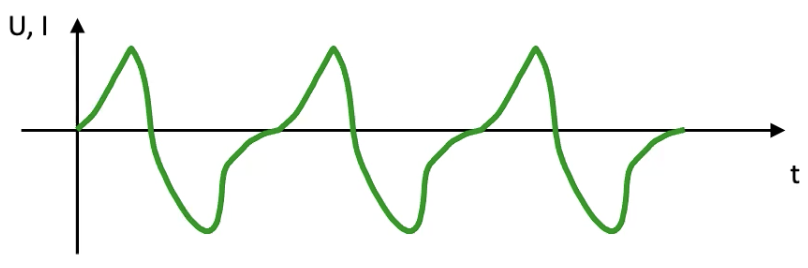
\includegraphics[width=0.5\textwidth]{chapters/chapter1/images/quelconque.png}
\end{center}
\textit{Remarque personelle - Le théorème de Fourier stipule que tout signal périodique peut être décomposé en une somme de signaux sinusoïdaux.}
\subsubsection{Exemples}
\textit{Parmis les exemples de signaux alternatifs et périodiques, on peut citer :} \\
\vspace{5px}
\begin{minipage}[htp]{0.45\textwidth}
\textbf{Signal Triangle} : Signal qui varie linéairement en fonction du temps. \\
\vspace{4ex}
\begin{center}
    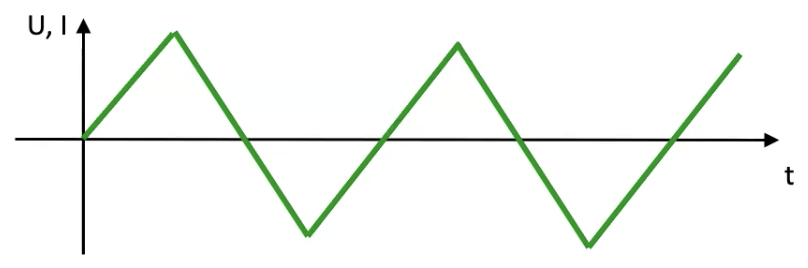
\includegraphics[width=\textwidth]{chapters/chapter1/images/triangle.png}
\end{center}
\end{minipage}
\hfill
\vline
\hfill
\begin{minipage}[htp]{0.45\textwidth}
\textbf{Signal Carré} : Signal qui varie de manière abrupte en fonction du temps. (eg. horloge d'un ordinateur)\\
\begin{center}
    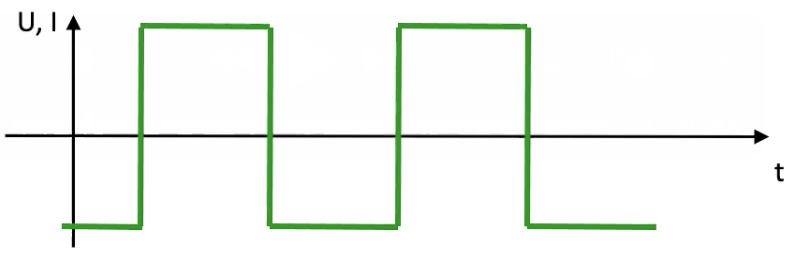
\includegraphics[width=\textwidth]{chapters/chapter1/images/carre.png}
\end{center}
\end{minipage}
\subsection{Signal Sinusoïdal}
\textit{On peut caractériser n'importe quel circuit analogique en utilisant des signaux sinusoïdaux.} \\
\textbf{Signal Sinusoïdal} : Signal qui varie de manière sinusoïdale en fonction du temps.

\begin{itemize}
    \item[-] \textbf{Valeur crête} : Amplitude maximale du signal, notée \( V_m \).
    \item[-] \textbf{Valeur crête-à-crête} : Différence entre la valeur maximale et la valeur minimale (eg. \( 2V_m \)).
    \item[-] \textbf{Valeur moyenne} : Moyenne du signal sur une période. Pour un signal sinusoïdal, elle est nulle.
    \item[-] \textbf{Valeur efficace (RMS)} : Représente la valeur d'une tension ou d'une intensité qui produirait le même effet électrique (puissance moyenne) qu'un signal continu. Elle est plus utile pour évaluer l'énergie réellement transmise par le signal.
\end{itemize}

\begin{center}
    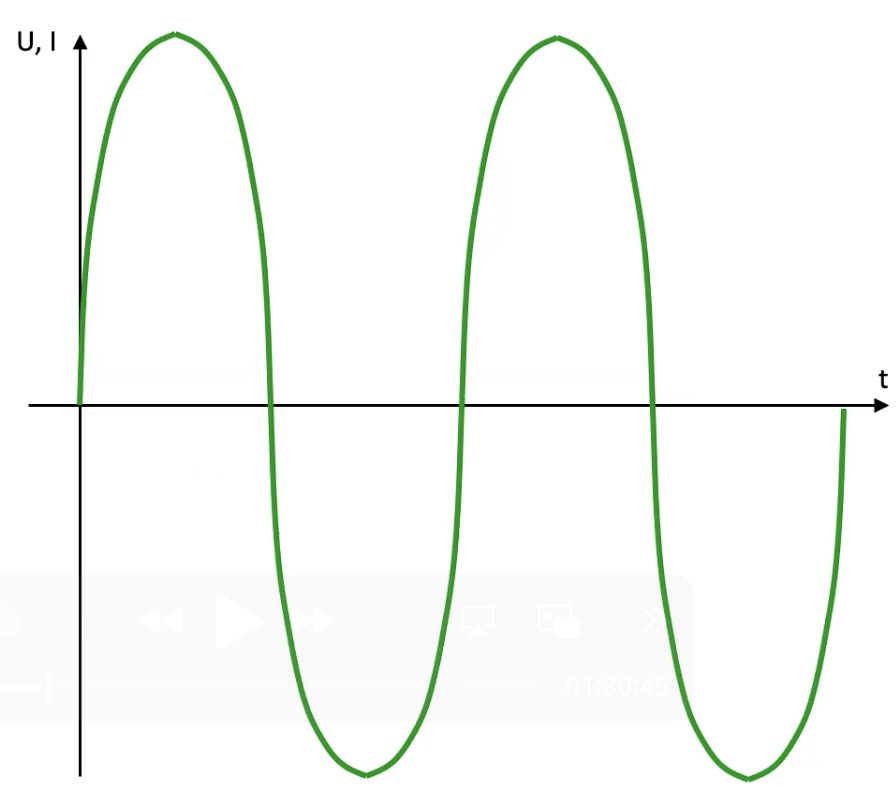
\includegraphics[width=0.3\textwidth]{chapters/chapter1/images/sinus.png}
\end{center}

\subsection{Création des signaux électriques}

Pour générer des signaux électriques, il est nécessaire d'utiliser des sources d'énergie, à savoir :

\vspace{10px}
\begin{minipage}[htp]{0.45\textwidth}
    \textbf{Source de tension :} $U_0$ \\
    \begin{center}
        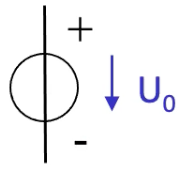
\includegraphics[width=0.32\textwidth]{chapters/chapter1/images/source_tension.png}
    \end{center}
\end{minipage}
\hfill
\vline
\hfill
\begin{minipage}[htp]{0.45\textwidth}
    \textbf{Source de courant :} $i$ \\
    \begin{center}
        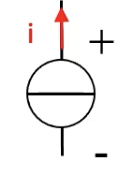
\includegraphics[width=0.25\textwidth]{chapters/chapter1/images/source_courant.png}
    \end{center}
\end{minipage}



\textit{Premières conventions: } \\
\begin{itemize}
    \item[-] Les \textbf{signaux continus} sont représentés par des lettres majuscules : $U$, $V$, $I$
    \item[-] Les \textbf{signaux variables} sont représentés par des lettres minuscules : $u(t)$, $v(t)$, $i(t)$, $u$, $v$, $i$
    \item[-] Le \textbf{courant d'électrons} est inversé par rapport au courant électrique.
\end{itemize}
